\documentclass{article}\usepackage[]{graphicx}\usepackage[]{color}
%% maxwidth is the original width if it is less than linewidth
%% otherwise use linewidth (to make sure the graphics do not exceed the margin)
\makeatletter
\def\maxwidth{ %
  \ifdim\Gin@nat@width>\linewidth
    \linewidth
  \else
    \Gin@nat@width
  \fi
}
\makeatother

\definecolor{fgcolor}{rgb}{0.345, 0.345, 0.345}
\newcommand{\hlnum}[1]{\textcolor[rgb]{0.686,0.059,0.569}{#1}}%
\newcommand{\hlstr}[1]{\textcolor[rgb]{0.192,0.494,0.8}{#1}}%
\newcommand{\hlcom}[1]{\textcolor[rgb]{0.678,0.584,0.686}{\textit{#1}}}%
\newcommand{\hlopt}[1]{\textcolor[rgb]{0,0,0}{#1}}%
\newcommand{\hlstd}[1]{\textcolor[rgb]{0.345,0.345,0.345}{#1}}%
\newcommand{\hlkwa}[1]{\textcolor[rgb]{0.161,0.373,0.58}{\textbf{#1}}}%
\newcommand{\hlkwb}[1]{\textcolor[rgb]{0.69,0.353,0.396}{#1}}%
\newcommand{\hlkwc}[1]{\textcolor[rgb]{0.333,0.667,0.333}{#1}}%
\newcommand{\hlkwd}[1]{\textcolor[rgb]{0.737,0.353,0.396}{\textbf{#1}}}%
\let\hlipl\hlkwb

\usepackage{framed}
\makeatletter
\newenvironment{kframe}{%
 \def\at@end@of@kframe{}%
 \ifinner\ifhmode%
  \def\at@end@of@kframe{\end{minipage}}%
  \begin{minipage}{\columnwidth}%
 \fi\fi%
 \def\FrameCommand##1{\hskip\@totalleftmargin \hskip-\fboxsep
 \colorbox{shadecolor}{##1}\hskip-\fboxsep
     % There is no \\@totalrightmargin, so:
     \hskip-\linewidth \hskip-\@totalleftmargin \hskip\columnwidth}%
 \MakeFramed {\advance\hsize-\width
   \@totalleftmargin\z@ \linewidth\hsize
   \@setminipage}}%
 {\par\unskip\endMakeFramed%
 \at@end@of@kframe}
\makeatother

\definecolor{shadecolor}{rgb}{.97, .97, .97}
\definecolor{messagecolor}{rgb}{0, 0, 0}
\definecolor{warningcolor}{rgb}{1, 0, 1}
\definecolor{errorcolor}{rgb}{1, 0, 0}
\newenvironment{knitrout}{}{} % an empty environment to be redefined in TeX

\usepackage{alltt}
\usepackage{natbib}
\usepackage{url}
\IfFileExists{upquote.sty}{\usepackage{upquote}}{}
\begin{document}

\title{Wordcloud Analysis of Dr. Jekyll and Mr. Hyde}
\author{Ron Richardson}
\maketitle

\begin{abstract}
This article contains the code and explanation of how to create a wordcloud using the text from Robert Louis Stevenson`s novel \textit{The Strange Case of Dr. Jekyll and Mr. Hyde}.
\end{abstract}

\section{Introduction}
A wordcloud is a type of visualization that shows the frequency of a word within a collection by changing the size of the word. The more frequently a word is used, the larger it shows up in the wordcloud.  In this article, we will be using R and RStudio to create a wordcloud.\footnote{What is Captain Blackbeard`s favorite programming language?  ARRRRRR}

In the spirit of Halloween, we have chosen the novel \textit{The Strange Case of Dr. Jekyll and Mr. Hyde} by Robert Louis Stevenson. It was written in 1886 and is available via Project Gutenberg, who graciously provide the text via their R package gutenberg \citep{Gutenberg}.

\section{Obtaining the Text}
To obtain the text, we must first import our libraries and find the text we want. For the purposes of this article, we have already searched for the text we want, but have included code to search by title.

\begin{knitrout}
\definecolor{shadecolor}{rgb}{0.969, 0.969, 0.969}\color{fgcolor}\begin{kframe}
\begin{alltt}
\hlkwd{library}\hlstd{(gutenbergr)}
\hlkwd{library}\hlstd{(dplyr)}
\hlkwd{library}\hlstd{(stringr)}

\hlcom{#search by title }
\hlkwd{gutenberg_works}\hlstd{(}\hlkwd{str_detect}\hlstd{(title,} \hlstr{'Jekyll'}\hlstd{))}
\end{alltt}
\begin{verbatim}
## # A tibble: 1 x 8
##   gutenberg_id                                       title
##          <int>                                       <chr>
## 1           42 The Strange Case of Dr. Jekyll and Mr. Hyde
## # ... with 6 more variables: author <chr>, gutenberg_author_id <int>,
## #   language <chr>, gutenberg_bookshelf <chr>, rights <chr>,
## #   has_text <lgl>
\end{verbatim}
\begin{alltt}
\hlcom{#store the text into a data frame of two columns}
\hlstd{jh}\hlkwb{<-}\hlkwd{gutenberg_download}\hlstd{(}\hlnum{42}\hlstd{,} \hlkwc{strip}\hlstd{=}\hlnum{TRUE}\hlstd{)}
\end{alltt}
\end{kframe}
\end{knitrout}

\section{Cleaning the Text}
Once we have downloaded our text, we want to remove any lines of text that contain information we don`t want to include in our wordcloud. This can contain information such as the label for each chapter, or the title page and author`s name. 

By looking at the first 20 rows, we can see the first 10 contain the title page. We can also se on row 11, how the chapter labels are formatted.  Using a regular expression, we can filter those rows out and remove them from our data frame.

\begin{knitrout}
\definecolor{shadecolor}{rgb}{0.969, 0.969, 0.969}\color{fgcolor}\begin{kframe}
\begin{alltt}
\hlcom{#remove title page}
\hlstd{jh}\hlkwb{<-}\hlstd{jh[}\hlnum{10}\hlopt{:}\hlkwd{dim}\hlstd{(jh),]}

\hlcom{#remove chapter labels}
\hlstd{jh}\hlkwb{<-}\hlstd{jh}\hlopt
  \hlkwd{filter}\hlstd{(}\hlkwd{str_detect}\hlstd{(jh}\hlopt{$}\hlstd{text,} \hlstr{"^\textbackslash{}\textbackslash{}d+\textbackslash{}\textbackslash{})"}\hlstd{)}\hlopt{==}\hlnum{FALSE}\hlstd{)}
\end{alltt}
\end{kframe}
\end{knitrout}

\section{Creating Words From Lines}
To create a wordcloud, we need to know the frequency of each word. Currently, our data is stored in lines, so we need to convert them. The tidytext package provides a great function to un-nest the words. This will break apart each line (the `text` column) into words, which we will store into a new dataframe.

\begin{knitrout}
\definecolor{shadecolor}{rgb}{0.969, 0.969, 0.969}\color{fgcolor}\begin{kframe}
\begin{alltt}
\hlkwd{library}\hlstd{(tidytext)}

\hlstd{words}\hlkwb{<-}\hlstd{jh}\hlopt
  \hlkwd{unnest_tokens}\hlstd{(word, text)}
\end{alltt}
\end{kframe}
\end{knitrout}

Once we have the words split apart, we want to remove any unnecessary words, such as indefinite articles (a, an, the). Again, the tidytext package provides a function that contains these words, called stop words.

\begin{knitrout}
\definecolor{shadecolor}{rgb}{0.969, 0.969, 0.969}\color{fgcolor}\begin{kframe}
\begin{alltt}
\hlstd{words}\hlkwb{<-}\hlstd{words}\hlopt
  \hlkwd{filter}\hlstd{(}\hlopt{!}\hlstd{(word} \hlopt \hlstd{stop_words}\hlopt{$}\hlstd{word))}
\end{alltt}
\end{kframe}
\end{knitrout}

\section{Creating the Wordcloud}
Now that we have a dataframe of just words, we need to get a count of how many times each word is used. Using the package dplyr, we can run a quick grouping query into a new dataframe.

\begin{knitrout}
\definecolor{shadecolor}{rgb}{0.969, 0.969, 0.969}\color{fgcolor}\begin{kframe}
\begin{alltt}
\hlstd{freq}\hlkwb{<-}\hlstd{words}\hlopt
  \hlkwd{group_by}\hlstd{(word)}\hlopt
  \hlkwd{summarize}\hlstd{(}\hlkwc{count}\hlstd{=}\hlkwd{n}\hlstd{())}
\end{alltt}
\end{kframe}
\end{knitrout}

The wordcloud package contains many customizations, but for the purposes of this article, we will keep it simple. We want to show the top 100 most used words in our wordcloud. There are over 3000 unique words in the novel, so generating the wordcloud could take a lengthy time if we included each one.

\begin{knitrout}
\definecolor{shadecolor}{rgb}{0.969, 0.969, 0.969}\color{fgcolor}\begin{kframe}
\begin{alltt}
\hlkwd{library}\hlstd{(wordcloud)}
\hlkwd{wordcloud}\hlstd{(freq}\hlopt{$}\hlstd{word, freq}\hlopt{$}\hlstd{count,} \hlkwc{max.words}\hlstd{=}\hlnum{100}\hlstd{)}
\end{alltt}
\end{kframe}
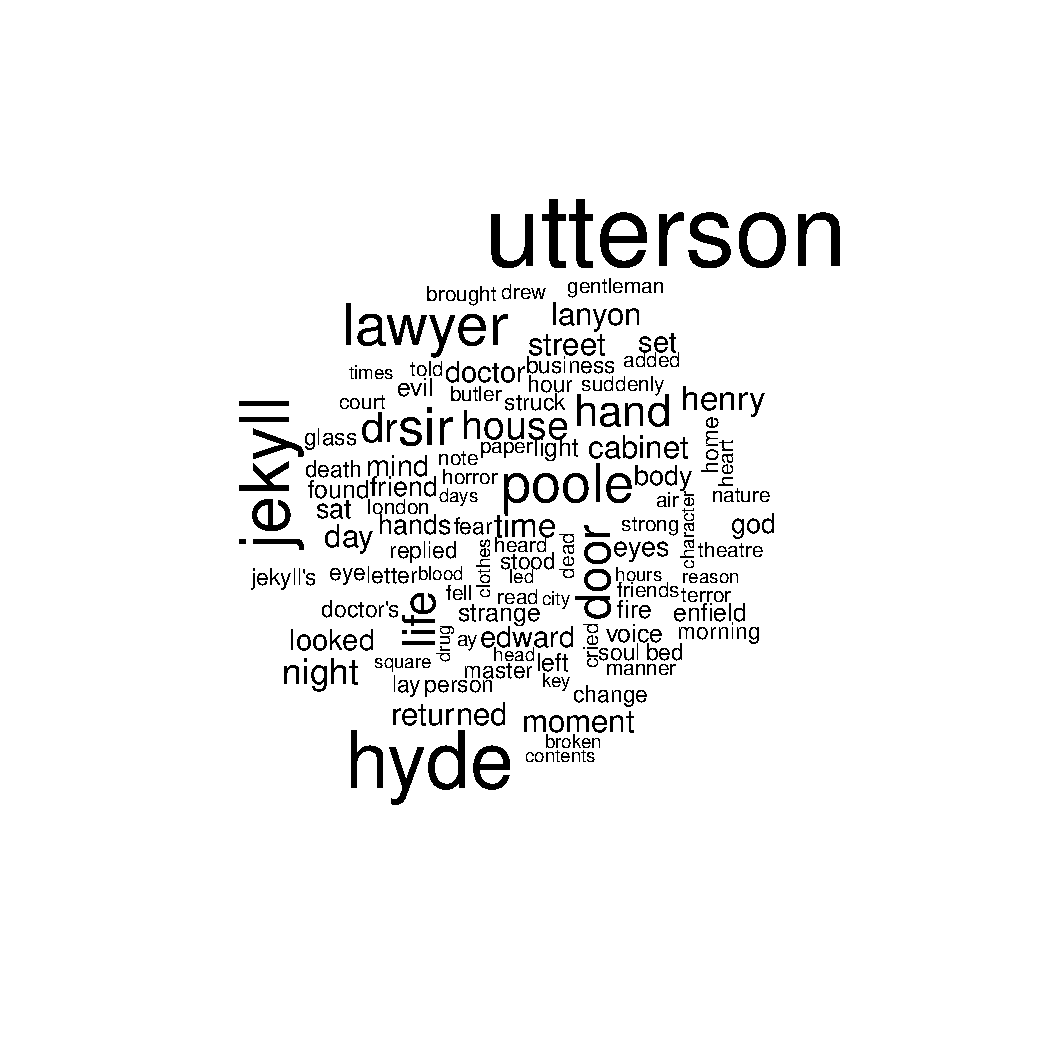
\includegraphics[width=\maxwidth]{figure/unnamed-chunk-6-1} 

\end{knitrout}

\section{Summary}
Looking at the wordcloud above, we can easily see which words are frequently used. In the case of this novel, it appears that the words `utterson`, `jekyll`, and `hyde` are the most frequent, with `poole`, `lawyer`, and `sir` coming in close behind.

Just from the wordcloud, we can surmise that `utterson` is a person`s name and `jekyll` and `hyde` are also character`s in the novel. Another hypothesis is that one of them is a laywer.

We can see now that generating a wordcloud is quite easy and can be a useful visualization to get a quick sense of what a collection of text is about.

\bibliographystyle{apa}
\bibliography{halloween}
\nocite{*}

\end{document}
